\documentclass[aps,twocolumn,secnumarabic,nobalancelastpage,amsmath,amssymb,
nofootinbib,superscriptaddress]{revtex4-1}


\usepackage{graphics}       % standard graphics specifications
\usepackage{graphicx}       % alternative graphics specifications
\usepackage{longtable}      % helps with long table options
\usepackage{url}            % for on-line citations
\usepackage{bm}             % special 'bold-math' package
\usepackage[ngerman]{babel} % deutsche Siblentrennung
\usepackage[utf8]{inputenc} % Umlaute

\def\andname{\hspace*{-0.5em},} % definiert die Trennung zwischen 2 Autoren neu

% Titelseite
\begin{document}
\title{Quantisierter Leitwert von Punktkontakten}
\author         {Ch. Egerland}
\email[Email: ]{egerlanc@physik.hu-berlin.de}
\author         {M. Pfeifer}
\email[Email: ]{max.pfeifer@physik.hu-berlin.de}
\affiliation    {Humboldt-Universität zu Berlin, Institut für Physik}
\date[Versuchsdatum: ]{22.06.2017}

%%%%%%%%%%%%%%%%%%%%%%%%%%%%%%%%%%%%%%%%%%%%%%%%%%%%%%%%%%%%%%%%%%%%%%%%%%%%%%%%
\begin{abstract}
Lorem ipsum dolor sit amet, consectetur adipiscing elit. Nam id facilisis ligula,
a ultrices nibh. Nullam suscipit tellus nec mauris fermentum, ornare luctus neque
tincidunt. Aenean commodo tincidunt varius. Phasellus faucibus metus non erat
consectetur bibendum. Duis et luctus risus, at egestas justo. Nunc eleifend lacus
ac laoreet scelerisque. Aenean cursus dignissim magna in ultrices. In eget nisl
quis nisi.
\end{abstract}


\maketitle



%%%%%%%%%%%%%%%%%%%%%%%%%%%%%%%%%%%%%%%%%%%%%%%%%%%%%%%%%%%%%%%%%%%%%%%%%%%%%%%%

\section{Theorie}

Der Leitwert ist das Inverse des Widerstandes und ist ein Maß dafür, wie gut ein
Material Strom leitet. Die Quantisierung des Leitwertes kann wie folgt erklärt
werden: Wir modellieren den Quantenpunktkontakt als ein effektives Kastenpotential
mit Breite $d_x$ und Dicke $d_y$. Es bilden sich senkrecht zur Bewegungsrichtung
stehende Elektronenwellen mit der Energie

  \begin{equation}
    E_{lm} = \frac{\pi^2 \hbar^2}{2 m_e} \left(\frac{l^2}{d_x^2}+\frac{m^2}{d_y^2} \right)
  \end{equation}

In Bewegungsrichtung haben wir unter den Voraussetzungen ein kontinuierliches
Energiespektrum mit $E_z = \hbar^2 k_z^2 / 2m_e$. Die Gesamtenergie der elektronischen
Zustände ist dann: $E_{ges} = E_{lm} + E_z$.
Die Zustandsdichte in einem eindimensionalen System ist gegeben durch:

  \begin{equation}
    D(E) dE = \frac{1}{\pi \hbar} \sqrt{\frac{m}{2 E}}dE
  \end{equation}

Bei Anlegen einer kleinen Spannung $dV$ folgt ein kleiner Strom $dI = e v dn$,
wobei $dn = D(E)dE$. Somit ist (mit $v = \sqrt{2E/m}$):

  \begin{equation}
    G = \frac{dI}{dV} = \frac{evD(E)dE}{dV} = \frac{e^2vD(E)dV}{dV} = \frac{2e^2}{h}
  \end{equation}






%%%%%%%%%%%%%%%%%%%%%%%%%%%%%%%%%%%%%%%%%%%%%%%%%%%%%%%%%%%%%%%%%%%%%%%%%%%%%%%%
\section{Experiment}

Das Experiment ist bebildert in \cite{skript11} erklärt und besteht im Wesentlichen
aus einem Lock-In-Verstärker an den zunächste zwei Transformatoren sowie die
Widerstandsbox angeschlossen sind. Nun wird überprüft, ob der gemessene Widerstand
dem angeschlossenen Widerstand entspricht. Die Abweichung vom Idealfall dient uns
dann als systematischer bzw. zufälliger Fehler (weiteres hierzu in Abschnitt III).
Nachdem die Widerstandsbox vermessen wurde wird der Messstab in flüssiges Helium
getaucht und entsprechend der Tabelle 2.1 in \cite{skript11} verkabelt. Nun messen
wir erneut die Ströme/Spannungen und ermitteln hieraus den Leitwert (weiteres
hierzu in Abschnitt III).



%%%%%%%%%%%%%%%%%%%%%%%%%%%%%%%%%%%%%%%%%%%%%%%%%%%%%%%%%%%%%%%%%%%%%%%%%%%%%%%%
\section{Daten und Analyse}
\subsection{Kalibrierung mittels Widerstandsbox}
Die Widerstandsbox mit ihren fest einstellbaren Widerständen bietet uns die
Möglichkeit den Messaufbau zu kalibrieren. Hierzu wurden für die festeingestellten
Widerstände 100 $\Omega$, 1 $k\Omega$, 10 $k\Omega$, 100 $k\Omega$ und 1 $M\Omega$
die Real- und Imaginärteile der Impedanz bei verschiedenen Spannungswerten ermittelt
und durch pythagoräische Addtion der Widerstand ermittelt. Als Fehler wurde auf der
Widerstandsbox $0.1\%$ für den Bereich $100\Omega - 10k\Omega$ und $1\%$ für den
Bereich $10k\Omega - 1M\Omega$ gegeben. Aus unseren Messdaten ergibt sich Abbildung
\ref{fig:box}

\begin{figure}[h]
  \centering
  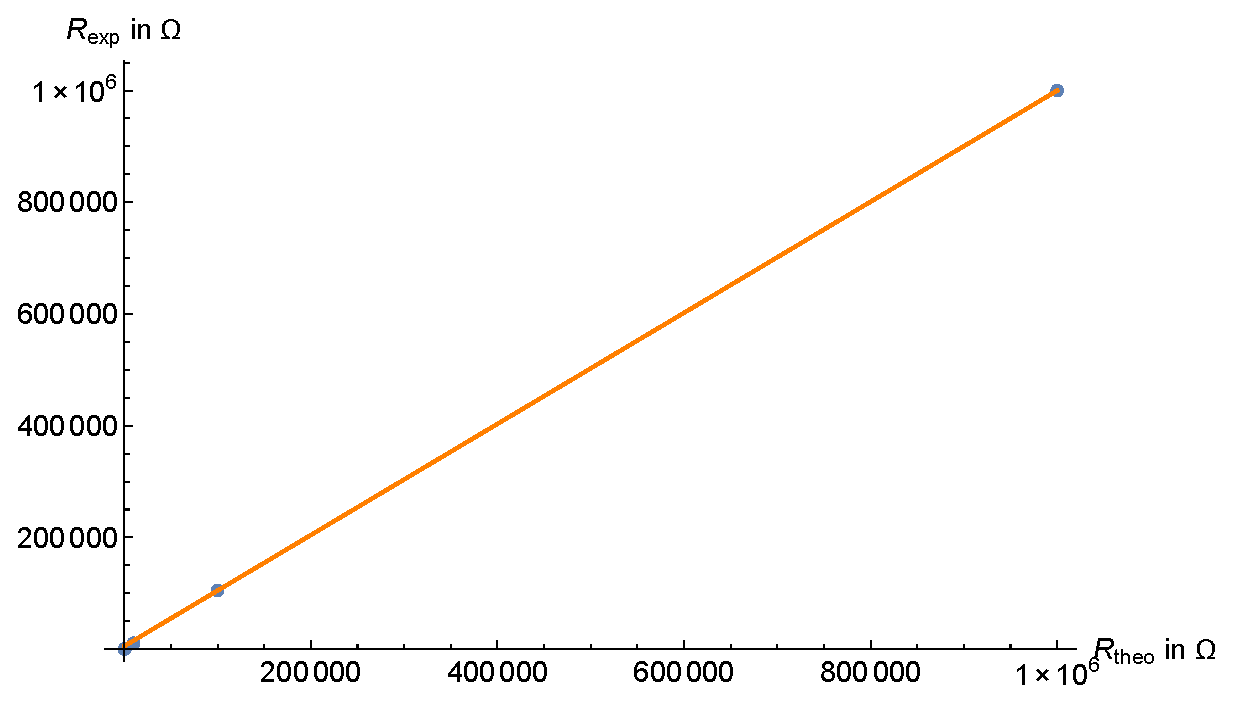
\includegraphics[width=0.5\textwidth]{Berechnung-Bilder/box.eps}
  \caption{Kalibrierung mit Widerstandsbox, lineare Regression}
  \label{fig:box}
\end{figure}




%%%%%%%%%%%%%%%%%%%%%%%%%%%%%%%%%%%%%%%%%%%%%%%%%%%%%%%%%%%%%%%%%%%%%%%%%%%%%%%%
\section{Schlussfolgerung}

Schlussoflgerung, sollten wir mal was von nem Buch oder so entnehmen nutzen wir:


\begin{quote}
  Ein Zitat mit Referenz auf das Buch\cite{melissinos1966}
\end{quote}

Lorem ipsum dolor sit amet, consectetur adipiscing elit. Nam id facilisis ligula,
a ultrices nibh. Nullam suscipit tellus nec mauris fermentum, ornare luctus neque
tincidunt. Aenean commodo tincidunt varius. Phasellus faucibus metus non erat
consectetur bibendum. Duis et luctus risus, at egestas justo. Nunc eleifend lacus
ac laoreet scelerisque. Aenean cursus dignissim magna in ultrices. In eget nisl
quis nisi.


%%%%%%%%%%%%%%%%%%%%%%%%%%%%%%%%%%%%%%%%%%%%%%%%%%%%%%%%%%%%%%%%%%%%%%%%%%%%%%%%
\bibliography{sample-paper}
\bibliographystyle{prsty}
\begin{thebibliography}{99}
\bibitem{skript11}S. F. Fischer et al. : F-Praktikumsversuch Quantisierter Leitwert von Punktkontakten (Versuchsskript) (2011)
\bibitem{wees88}B. J. van Wees et al. : Quantized Conductance of Point Contacts in a Two-Dimensional Electron Gas, Physical Review Letters Vol. 60 Nr.9 (1988)
\bibitem{wharam88}D. A. Wharam et al. : One-dimensional transport and the quantisation of the ballistic resistance Verlag, Phys. C: Solid State Phys. 21  (1988)
\bibitem{apetrii04}Gabriela Apetrii : Quantum point contacts with one and two vertical modes fabricated with an atomic force microscope, Dissertation (2004)
\bibitem{vanhouten96}Henk van Houten et al. :  Quantum Point Contacts, Physics Today July S. 22–27, (1996)
\bibitem{knop07}Michael H. Knop :  Ballistische Gleichrichtung in asymmetrischen elektronischen Wellenleiterkreuzen, Dissertation (2007)
\bibitem{fischer02}S. F. Fischer et al. :  Control of the confining potential in ballistic constrictions using a persistent charging effect, Applied Physics Letters Vol. 81 Nr.15 (2002)
\bibitem{apetrii02}G. Apetrii et al. :  Influence of processing parameters on the transport properties of quantum point contacts fabricated with an atomic force microscope, Institute of Physics Publishing Semicond. Sci. Technol. 17 S. 735–739 (2002)
\end{thebibliography}


%%%%%%%%%%%%%%%%%%%%%%%%%%%%%%%%%%%%%%%%%%%%%%%%%%%%%%%%%%%%%%%%%%%%%%%%%%%%%%%%
\clearpage
\appendix

\section{Sonstiges}
Hier sehen wir einen Beispiel Anhang und so könnte man Code in Latex einbinden:
\begin{verbatim}
> mkdir ~/8.13
> mkdir ~/8.13/papers
> mkdir ~/8.13/papers/template
> cd ~/8.13/papers/template
\end{verbatim}


%%%%%%%%%%%%%%%%%%%%%%%%%%%%%%%%%%%%%%%%%%%%%%%%%%%%%%%%%%%%%%%%%%%%%%%%%%%%%%%%


\end{document}
